%%%%%%%%%%%%%%%%%%%%%%%%%%%%%%%%%%%%%%%%%%%%%%%%%%%%%%%%%%%
% CLASS AND PACKAGES
%%%%%%%%%%%%%%%%%%%%%%%%%%%%%%%%%%%%%%%%%%%%%%%%%%%%%%%%%%%
\documentclass[ 12pt, a4paper, oneside ]{memoir}

\usepackage{graphics}
\usepackage{dcolumn}
\usepackage{longtable}
\usepackage{graphicx}
\usepackage{chemfig}
\usepackage{amsmath}
\usepackage{float}
\usepackage{comment}
\usepackage{soul}
\usepackage[flushleft]{threeparttable}
\usepackage{multirow}

\usepackage{booktabs}
\usepackage{titlesec}

\usepackage[T1]{fontenc}
% Necessary for _ to be displayed correctly
\usepackage{etoolbox}
% Necessary for \csuse, \csdef, \ifcsdef and \forcsvlist
\usepackage{tabularx}
% For code snipets
\usepackage{listings}

%For Hyperlinks in TOC
\usepackage[hidelinks]{hyperref}
\usepackage{xcolor}
\hypersetup{
    colorlinks,
    linkcolor={black!80!black},
    citecolor={blue!50!black},
    urlcolor={blue!50!black}
}

% Custom colors for LIO variables.
\definecolor{liopurple}{RGB}{139, 94, 145}
\definecolor{liogreen}{RGB}{55, 117, 53}
\definecolor{lioblue}{RGB}{53, 99, 160}
\definecolor{lioteal}{RGB}{97, 191, 181}
\newcommand{\textliovar}[1]{\textbf{\textit{\textcolor{liogreen}{#1}}}}

%%%%%%%%%%%%%%%%%%%%%%%%%%%%%%%%%%%%%%%%%%%%%%%%%%%%%%%%%%%%
% Package for flow diagrams

\usepackage{tikz}

\usetikzlibrary{shapes.geometric, arrows}

% Define block styles

\tikzstyle{startstop} = [ rectangle, rounded corners,
   minimum width=3cm, minimum height=1cm, text centered,
draw=black, fill=blue!30 ]

\tikzstyle{element} = [ rectangle, rounded corners,
   minimum width=3cm, minimum height=1cm, text centered,
draw=black, text width=4cm, fill=yellow!30 ]

\tikzstyle{decision} = [ diamond, minimum width=3cm,
   minimum height=1cm, text centered, draw=black,
fill=green!30 ]

\tikzstyle{yes} = [ circle, minimum size=1cm,
text centered, draw=black, fill=red!30 ]

\tikzstyle{no} = [ circle, minimum size=1cm,
text centered, draw=black, fill=red!30 ]

\tikzstyle{arrow} = [ thick, ->, >=stealth ]

%%%%%%%%%%%%%%%%%%%%%%%%%%%%%%%%%%%%%%%%%%%%%%%%%%%%%%%%%%%%


%%%%%%%%%%%%%%%%%%%%%%%%%%%%%%%%%%%%%%%%%%%%%%%%%%%%%%%%%%%
% GENERAL SETTINGS AND MACROS
%%%%%%%%%%%%%%%%%%%%%%%%%%%%%%%%%%%%%%%%%%%%%%%%%%%%%%%%%%%
\setulmarginsandblock{3.0cm}{3.0cm}{*}
\setlrmarginsandblock{3.5cm}{2.0cm}{*}

%\setlength{\textfloatsep}{1pt}
%\setlength{\intextsep}{0.1pt}
\renewcommand{\baselinestretch}{1.5}

\checkandfixthelayout 

\newcommand{\Hquad}{\hspace{0.5em}}

%%%%%%%%%%%%%%%%%%%%%%%%%%%%%%%%%%%%%%%%%%%%%%%%%%%%%%%%%%%
% INCLUDE CONTENT
%%%%%%%%%%%%%%%%%%%%%%%%%%%%%%%%%%%%%%%%%%%%%%%%%%%%%%%%%%%
\title{LIO User Guide}
\author{NaN}

\begin{document}

\frontmatter
%%%%%%%%%%%%%%%%%%%%%%%%%%%%%%%%%%%%%%%%%%%%%%%%%%%%%%%%%%%%%%%%%%%%%%%%%%%%%%%%
\thispagestyle{empty}
\parindent=0cm{

    \par
    
\includegraphics[scale=0.3,keepaspectratio=true]{../fig/logo_fcen.png}
    \hfill
    
\includegraphics[scale=0.2,keepaspectratio=true]{../fig/logo_inquimae.png}
    \par

    \rule{\linewidth}{0.5ex}
    \begin{center}
       
\includegraphics[scale=0.5,keepaspectratio=true]{../fig/logo_lio.jpg}
    \end{center}
    \rule{\linewidth}{0.5ex}
    
    \begin{center}
    \vspace*{\stretch{1}}
    \sffamily\bfseries\Huge{LIO User Guide} \\
    \vspace*{\stretch{1}}
    \sffamily\bfseries\large{V 1.11} \\
    \vspace*{\stretch{1}}
    \sffamily\LARGE{January, 2020} \\
    \vspace*{\stretch{1}}
    \end{center}

}
\cleardoublepage
%
%
%%%%%%%%%%%%%%%%%%%%%%%%%%%%%%%%%%%%%%%%%%%%%%%%%%%%%%%%%%%%%%%%%%%%%%%%%%%%%%%%
\thispagestyle{empty}
\begin{center}
%\vspace*{\stretch{1}}
\sffamily\bfseries\Huge{Version Developers} \\
%\vspace*{\stretch{9}}
\end{center}

%%%%%%%%%%%%%%%%%%%%%%%%%%%%%%%%%%%%%%%%%%%%%%%%%%%%%%%%%%%%%%%%%%%%%%%%%%%%%%%%

\cleardoublepage
\tableofcontents
\newpage

\mainmatter
%\addtocontents{toc}{\protect\newpage}
%%%%%%%%%%%%%%%%%%%%%%%%%%%%%%%%%%%%%%%%%%%%%%%%%%%%%%%%%%%%
\chapter{Introduction}
%%%%%%%%%%%%%%%%%%%%%%%%%%%%%%%%%%%%%%%%%%%%%%%%%%%%%%%%%%%%
\section{What is LIO?}

Welcome to the LIO project! LIO is a library that can
perform electronic structure calculations using density
functional theory. 


\section{Instalation}

If you are reading this manual, you probably already have
a version of lio ready to compile. If you don't, or if
you want to make sure you have the most up-to-date version
of the code, all you need to do is either download it
from the git repository online or use git to clone a copy.

For the first option, go to
\textbf{\textit{\href
{https://github.com/MALBECC/lio}
{https://github.com/MALBECC/lio}
}}
and click on the green button that says 
\textit{clone or download}
and click on \textit{Download ZIP}.

For the second one, you can directly run the following
command:

\lstset{language=bash, keywordstyle=\color{violet}, 
morekeywords={clone}}
\begin{lstlisting}
   git clone https://github.com/MALBECC/lio.git .
\end{lstlisting}


\subsection{Pre-requisites}
In addition to an UNIX-like OS, fortran and c++ compilers,
LIO depends on LAPACK \textbf{\textit{\href{http://www.netlib.org/lapack/}
{LAPACK}}} and BLAS libraries for linear algebra calculations.
In addition, \textbf{\textit{\href{https://developer.nvidia.com/cuda-downloads}
{CUDA 6.5 or higher}}} is required for GPU calculations,
which unleash LIO's true potential. As of the writing of
this manual, LIO has not yet been tested with CUDA 9.0.

In addition, \textbf{\textit{\href{https://tddft.org/programs/libxc/}
{libxc}}} is required for its usage, although said library
is CPU-only. This is entirely optional as LIO can run
without libxc, using only the PBE functional.

\subsection{Compilation}

By default, LIO compiles with GPU options enabled. It is highly
recommended to specify the GPU architecture as a compilation
option, since the compiler performs additional enhancements.
After compilation, LIOHOME environment variable should be set
to the current LIO installation directory:

\lstset{language=bash, keywordstyle=\color{violet}, 
morekeywords={export}}
\begin{lstlisting}
   export LIOHOME=/dir/to/lio/
\end{lstlisting}

For a CPU-only compilation, use:

\lstset{language=bash, keywordstyle=\color{violet}, 
morekeywords={make}}
\begin{lstlisting}
   make cuda=0
\end{lstlisting}

If INTEL compilers are present, they can be used by setting
the \textit{intel} option to 1, or to 2 if INTEL MKL usage is
also desired. 

\lstset{language=bash, keywordstyle=\color{violet}, 
morekeywords={make}}
\begin{lstlisting}
   make intel=2
\end{lstlisting}

The following is a list of available compilation and their meanings.
They can be used in any combination possible (including several GPU
architectures for greater compatibility). For example, the default
LIO compilation could be written as:

\lstset{language=bash, keywordstyle=\color{violet}, 
morekeywords={make}}
\begin{lstlisting}
   make cuda=2 sm30=1 sm52=1 sm61=1
\end{lstlisting}

%%%%%%%%%%%%%%%%%%%%%%%%%%%%%%%%%%%%%%%%%%%%%%%%%%%%%%%%%%%%
\begin{Spacing}{1.0}
\begin{longtable}{ p{.25\textwidth} p{.70\textwidth} }

   \toprule
   \textbf{Variable} & Description \\*
   \midrule \\*
   \endhead

   \bottomrule
   \caption{Compilation options}
   \endfoot

   \textbf{cuda}
   &  \textit{default cuda=2}
   \\*\textit{0, 1, 2}
   & Sets the level of GPU dependencies. cuda=0 means a 
   CPU-only compilation, =1 enables GPU, and =2 includes
   CUBLAS usage for linear algebra operations. \\* \\

   \textbf{intel}
   &  \textit{default intel=0}
   \\*\textit{0, 1, 2}
   & Sets the usage of INTEL compilers. intel=0 means only
   GNU compilers, =1 means INTEL, and =2 uses INTEL MKL 
   instead of BLAS/LAPACK routines. \\* \\

   \textbf{precision}
   &  \textit{default precision=0}
   \\*\textit{0, 1}
   & Sets level of precision in XC calculations. By default
   LIO uses mixed precision; precision=1 sets everything in
   double precision. This is specially useful when attempting
   high-precision geometry optimizations.\\* \\

   \textbf{analytics}
   &  \textit{default analytics=0}
   \\*\textit{0, 1, 2, 3}
   & Setting analytics = 1 specifies a profiling compilation,
   while analytics = 2 and 3 set higher levels of debugging
   information (for usage with gdb, for example).
   \\* \\

   \textbf{smXX}
   &  \textit{default sm30=1 sm52=1 sm61=1}
   \\*\textit{0, 1}
   & Sets a specific GPU architecture for compilation. 
   Available options are sm30, sm35 (Kepler, CUDA $\geq$ 
   5.0), sm50, sm52 (Maxwell and GeForce 980, CUDA $\geq$
   6.5), sm60 and sm61 (Pascal and GeForce 1080, CUDA $\geq$
   8.0).
   \\* \\

\end{longtable}
\end{Spacing}
%%%%%%%%%%%%%%%%%%%%%%%%%%%%%%%%%%%%%%%%%%%%%%%%%%%%%%%%%%%%


\subsection{MD-Engine Interfacing}
LIO can be linked with  \textbf{\textit{\href{http://ambermd.org/index.php}
{AMBER}}}, our own \textbf{\textit{\href{https://github.com/MALBECC/gromacs}
{GROMACS fork}}}, our own \textbf{\textit{\href{https://github.com/MALBECC/hybrid}
{HYBRID}}} code for QM/MM calculations.

In all three cases, the LIOHOME environment variable should be
set to the current LIO installation directory. In addition
to this section, please refer to each of the software packages'
installation manual for further clarifications.

In order to compile AMBER with LIO, AMBER should be compiled
after LIO with the following options set:

\lstset{language=bash, keywordstyle=\color{violet}, 
morekeywords={make, export}}
\begin{lstlisting}
   export AMBERHOME=/dir/to/amber/
   ./configure -lio -noX11 -netcdfstatic gnu
   make clean
   make install
\end{lstlisting}

For a GROMACS-LIO compilation, GROMACS should be compiled 
after LIO with the following options:

\lstset{language=bash, breaklines=true, breakatwhitespace=true,
showstringspaces=false, stringstyle=\color{olive},
keywordstyle=\color{violet}, morekeywords={cmake, make}}
\begin{lstlisting}
   cd gromacs_compilation_directory/
   cmake gromacs_src_dir/ -DGMX_QMMM=1 -DGMX_QMMM_PROGRAM="lio" -DLIO_LINK_FLAGS="-L/usr/lib -L/usr/lib64 -L$LIOHOME/g2g -L$LIOHOME/lioamber -lg2g -llio-g2g" -DGMX_GPU=0 -DGMX_THREAD_MPI=0
   make
   make install
\end{lstlisting}

\section{Tips and tricks - Optimizing your runs}


%%%%%%%%%%%%%%%%%%%%%%%%%%%%%%%%%%%%%%%%%%%%%%%%%%%%%%%%%%%%


%\addtocontents{toc}{\protect\newpage}
%%%%%%%%%%%%%%%%%%%%%%%%%%%%%%%%%%%%%%%%%%%%%%%%%%%%%%%%%%%%
\chapter{General Settings}
%%%%%%%%%%%%%%%%%%%%%%%%%%%%%%%%%%%%%%%%%%%%%%%%%%%%%%%%%%%%

In this chapter we will describe the basic settings for running the code.
These will be necessary or useful for any of the features of the code
that you might be interested in using.

%%%%%%%%%%%%%%%%%%%%%%%%%%%%%%%%%%%%%%%%%%%%%%%%%%%%%%%%%%%%
\section{General System Description}

\begin{Spacing}{1.0}
   \begin{longtable}{ p{.25\textwidth} p{.70\textwidth} }
   
      \toprule
      \textbf{Variable} & Description \\*
      \midrule \\*
      \endhead
   
      \bottomrule
      \caption{General setup}
      \endfoot

       natom  & $ integer = 0 $ \\
       & Sets the number of atoms only in the QM region. This is ignored when
       calling LIO from another MM engine.\\
       \\
       nsol   & $ integer = 0 $ \\
       & Sets the number of "solvent" atoms, meaning atoms in the MM region. 
       This is also ignored when calling LIO externally. \\
       \\
       charge & $ integer = 0 $ \\
       & Sets the total charge for the QM region. \\
       \\
       OPEN   & $ logical = .false. $\\
       & Indicates whether an open-shell calculation should be performed.\\
       \\
       nUnp   & $ integer = 0 $ \\
       & Indicates the number of unpaired electrons for an open-shell calculation, 
       in a closed-shell calculation this variable is ignored. Keep in mind that 
       the number of unpaired electrons is NOT the multiplicity, rather nUnp = Mult+1.\\
       \\

   \end{longtable}
\end{Spacing}


%%%%%%%%%%%%%%%%%%%%%%%%%%%%%%%%%%%%%%%%%%%%%%%%%%%%%%%%%%%%
\section{Common Inputs and Outputs}

\begin{Spacing}{1.0}
   \begin{longtable}{ p{.25\textwidth} p{.70\textwidth} }
   
      \toprule
      \textbf{Variable} & Description \\*
      \midrule \\*
      \endhead
   
      \bottomrule
      \caption{Common inputs and outputs}
      \endfoot

      style  & $ logical = .false. $ \\
      & Activates a more stylish version of the output. \\
      \\
      verbose & $ integer = 0 $ \\
      & Sets verbose level for output. \\
      &     0 = Nothing is printed save for a small LIO start message.\\
      &     1 = only the input namelist and the final convergence results \\
      &         are printed.\\
      &     2 = information for each iteration is added.\\
      &     3 = GPU module information is added.\\
      &     4 = additional miscellaneous information is printed.\\
      \\
      writeXYZ & $ logical = .false. $\\
      & Writes and xyz file containing the QM region, using the filename
      specified in fcoord. This file is written in each of the MD steps 
      when LIO is used with AMBER/GROMACS/HYBRID. \\
      \\
      fCoord & $ character*20 = 'qm.xyz' $\\
      & Output file containing the QM region. \\
      \\
      timers & $ integer = 0 $ \\
      & Sets the timer level for benchmarking and profiling. \\
      &     0 = no timers. \\
      &     1 = only timers in certain subroutines. \\
      &     2 = full timer summary. \\
      \\
      dBug   & $ logical = .false. $\\
      & Checks for NaNs in Fock and Rho matrices.\\
      \\
      gaussian\_convert & $ logical = .false. $ \\
      & Reads an electron density from Gaussian09 as starting guess. 
      This feature is still experimental. \\
      \\
      print\_coeffs   & $ logical = .false. $\\
      & Prints coefficients and energies for each molecular orbital. \\
      \\      
      VCInp & $ logical = .false. $ \\
      & Reads a MO coefficient restart from frestartin.\\
      \\
      restart\_freq & $ integer = 1 $ \\
      & Writes a MO coefficient restart every restart\_freq iterations into 
      frestart.\\
      \\
      frestart & $ char*20 = 'restart.out' $ \\
      & Name of the output density or coefficient restart file. \\
      \\
      frestartin & $ char*20 = 'restart.in' $ \\
      & Name of the input density or coefficient restart file. \\
      \\
      rst\_dens & $ integer = 0 $ \\
      & When rst\_dens >= 1, the restart read by VCInp must be a density
      matrix (not coefficient matrix) restart. Likewise, when rst\_dens = 2,
      the restart written with restart\_freq is a density matrix restart
      (instead of a coefficient matrix restart). \\
      \\
   \end{longtable}
\end{Spacing}


%%%%%%%%%%%%%%%%%%%%%%%%%%%%%%%%%%%%%%%%%%%%%%%%%%%%%%%%%%%%
\section{Properties Calculations}


\begin{Spacing}{1.0}
   \begin{longtable}{ p{.25\textwidth} p{.70\textwidth} }
   
      \toprule
      \textbf{Variable} & Description \\*
      \midrule \\*
      \endhead
   
      \bottomrule
      \caption{Common inputs and outputs}
      \endfoot

      writeForces  & $ logical = .false. $ \\
      & Performs forces calculation and prints the result to a file named
      "forces". \\
      \\
      dipole & $ logical = .false. $ \\
      & Performs dipole calculation and prints the result to a file named
      "dipole". \\
      \\
      mulliken & $ logical = .false. $ \\
      & Performs a Mulliken population analysis and outputs the result to
      a file called "mulliken".\\
      lowdin & $ logical = .false. $ \\
      & Performs a Lowdin population analysis and outputs the result to
      a file called "mulliken".\\
      fukui & $ logical = .false. $ \\
      & Calculates the condensed-to-atoms Fukui function for the system, 
      calculating the spin-polarized version in open-shell systems.\\
   \end{longtable}
\end{Spacing}

%%%%%%%%%%%%%%%%%%%%%%%%%%%%%%%%%%%%%%%%%%%%%%%%%%%%%%%%%%%%
\section{GPU Options}

These options affect the calculations in the GPU module. For the exchange
correlation integrals, the integration grid is separated into cubes and spheres,
with the smaller cubes (less points per cube) being calculated in CPU while the
rest is calculated in GPU. Most of these options should be tweaked for optimal
performance in a given system.

\begin{Spacing}{1.0}
   \begin{longtable}{ p{.35\textwidth} p{.60\textwidth} }
   
      \toprule
      \textbf{Variable} & Description \\*
      \midrule \\*
      \endhead
   
      \bottomrule
      \caption{GPU Module Options}
      \endfoot
   
      \textbf{gpu\_level}
      &  \textit{default = 4}
      \\*\textit{integer}
      & Determines which calculations are performed by the GPU, only
      available when compiled with cuda > 0.\\*
      &     0/1 = only exchange-correlation integrals.\\
      &     2 = adds QM/MM interaction energies and gradients.\\
      &     3 = adds Coulomb energies and gradients.\\
      &     4 = adds nuclear attraction energies and gradients.\\
      &     5 = adds Coulomb basis fitting energies and gradients.\\
      \\
   
      \textbf{max\_function\_exponent}
      &  \textit{default = 10}
      \\*\textit{integer}
      & Ignores functions with $\lvert exponent \rvert > 
      max\_function\_exponent$. This is only for the exchange-correlation
      calculations.\\* \\
   
      \textbf{little\_cube\_size}
      &  \textit{default = 8.0d0}
      \\*\textit{double precision}
      & Small cube-type point group size (in Angstrom).\\* \\
   
      \textbf{min\_points\_per\_cube}
      &  \textit{default = 1}
      \\*\textit{integer}
      & Minimum number of grid points in a cube.\\* \\
   
      \textbf{assign\_all\_functions}
      &  \textit{default = .false. }
      \\*\textit{logical}
      & Calculate \textbf{all} functions (ignores $max\_function\_exponent$).
      This is intended only as a debug option and its usage is not recommended.\\* \\
   
      \textbf{sphere\_radius}
      &  \textit{default = 0.6d0}
      \\*\textit{double precision}
      & Radius of the sphere-type point groups. 0 means there are no sphere-type
      groups, 1 means all points are contained in sphere-type groups.\\* \\
   
      \textbf{remove\_zero\_weights}
      &  \textit{default = .true. }
      \\*\textit{logical}
      & Discard functions for those whose weight is zero
      (.false. option only remains as a debug option).
      \\* \\
   
      \textbf{energy\_all\_iterations}
      &  \textit{default = .false. }
      \\*\textit{logical}
      & Calculate Exc energy in all SCF iterations. Usually, XC energy is only
      calculated in the final step in order to accelerate calculations. \\* \\
   
      \textbf{free\_global\_memory}
      &  \textit{default = 0.0d0}
      \\*\textit{double precision}
      & Fraction of global GPU memory available for the calculation
      (1 means 100\%).\\* \\
   
   
   \end{longtable}
   \end{Spacing}
%%%%%%%%%%%%%%%%%%%%%%%%%%%%%%%%%%%%%%%%%%%%%%%%%%%%%%%%%%%%


%\addtocontents{toc}{\protect\newpage}
%%%%%%%%%%%%%%%%%%%%%%%%%%%%%%%%%%%%%%%%%%%%%%%%%%
\chapter{Model Hamiltonian}
%%%%%%%%%%%%%%%%%%%%%%%%%%%%%%%%%%%%%%%%%%%%%%%%%%


%%%%%%%%%%%%%%%%%%%%%%%%%%%%%%%%%%%%%%%%%%%%%%%%%%
\section{Density Functional Theory}
\begin{Spacing}{1.0}
   \begin{longtable}{ p{.25\textwidth} p{.70\textwidth} }
   
      \toprule
      \textbf{Variable} & Description \\*
      \midrule \\*
      \endhead
   
      \bottomrule
      \caption{DFT Hamiltonian}
      \endfoot
   
      iexch & $ integer = 9 $ \\
      & Identifies the exchange-correlation potential to use with the
      calculation when not using libxc. Iexch=9 is the only option
      currently available.\\
      \\
   
      use\_libxc & $ logical = .false. $ \\
      & Activates the use of libxc version of the XC potential.\\
      \\
   
      ex\_functional\_id & $ integer = none $ \\
      & Exchange functional to use with libxc. Please refer to libxc 
      for the desired functional.\\
      \\
   
      ec\_functional\_id & $ integer = none $ \\
      & Correlation functional to use with libxc. Please refer to libxc 
      for the desired functional.\\
      \\
   
      int\_basis & $ logical = .false. $ \\
      & If true, looks for the internal basis indicated in variables $basis\_set$
      and $fitting\_set$ (defaults are $'DZVP'$ and$'DZVP Coulomb Fitting'$. If
      false, an external basis file must be provided in the keyword $basis\_set$.\\
      \\
   
      basis\_set & $ char*20 = 'DZVP' $ \\
      & Name of the basis set used in the calculation when $int\_basis$ is set
      to true. If not, it is the name of the file containing the custom basis
      data. \\
      \\
   
      fitting\_set & $ char*100 = 'DZVP Coulomb Fitting' $ \\
      & Name of the fitting set used in the calculation when $int\_basis$ is
      set to true.\\
      \\   
   
      n\_ghosts & $ integer = 0 $ \\
      & Number of ghost atoms. Ghost atoms are considered for the basis functions
      of the system, but they are considered as having zero electrons and zero
      nuclear charge. \\
      \\
   
      ghost\_atoms & $ integer = 0 $ \\
      & A list containing the atom indeces for those considered ghost\_atoms. 
      For example, $ghost\_atoms = 1,2 $ considers the first and second atoms
      as ghosts. \\
      \\
   
      rmax & $ double = 16.0d0 $ \\
      & Maximum exponent in 3-center integrals. If exponent
      is greater than $rmax$, the current term is ignored. \\
      \\

      rmaxs & $ double = 5.0d0 $ \\
      & If the exponent in 3-center integral is within
      $rmax$ and $rmaxs$, calculation is performed using
      double precision. If it is between 0 and $rmaxs$, 
      the calculation is performed in single precision.
      This is ignored when using the AINT module. \\
      \\
   
      iGrid & $ integer = 2 $ \\
      & Grid type when iterating through SCF. Available 
      values are 1 (less dense) and 2 (more dense).\\
      \\
   
      iGrid2 & $ integer = 2 $ \\
      & Grid type for the final density calculation in
      SCF. Available values are 1 (less dense) and 2
      (more dense).\\
      \\
   \end{longtable}
   \end{Spacing}

%%%%%%%%%%%%%%%%%%%%%%%%%%%%%%%%%%%%%%%%%%%%%%%%%%
\section{Convergence Options}
\begin{Spacing}{1.0}
   \begin{longtable}{ p{.25\textwidth} p{.70\textwidth} }
   
      \toprule
      \textbf{Variable} & Description \\*
      \midrule \\*
      \endhead
   
      \bottomrule
      \caption{BO-MD useful settings.}
      \endfoot
         initial\_guess & $ integer = 0 $ \\
         & Selects the method for calculating a starting guess. When set to
         0, the initial guess comes from the 1-electron integrals, while
         setting it to 1 performs an Aufbau-like initial guess. \\
         \\
         nMax & $ integer = 100 $ \\
         & Maximum number of SCF iteration steps.\\
         \\
         told  & $ double \Hquad precision = 1.0d-6 $ \\
         & Criterium for the maximal square deviation of the density matrix to 
         consider that the convergence has been achieved. \\
         \\
         etold & $ double \Hquad precision = 1.0d0 $ \\
         & Criterium for the maximal energy difference to consider that the
         convergence has been achieved. \\
         \\
         DIIS  & $ logical = .true. $\\
         & Uses DIIS algorithm for convergence. If disabled, it tries to
         converge using a damping factor between iterations. \\
         \\
         nDIIS & $ integer = 30 $ \\
         & Number of matrices considered for DIIS. Only change this if you know
         what you are doing. \\
         \\
         gold & $ double \Hquad precision = 1.0d+1 $\\
         & Determines the weight of the previous density matrix in the linear 
         combination with the new one when using the damping convergence method
         ( DIIS = .false. / hybrid\_converg ).\\
         \\
         hybrid\_converg & $ logical = .false. $\\
         & Uses the hybrid convergence algorithm: it starts using the damping
         factor, and after a threshold is met, changes to DIIS. This method
         usually gives the best results in cases which are difficult to 
         converge.\\
         \\
         good\_cut & $ double \Hquad precision = 1.0d-3 $\\
         & Sets the threshold to start DIIS when activating hybrid convergence
         (hybrid\_converg = 1). When the mean square deviation for the density
         matrix between two iteration steps reaches this threshold, DIIS is
         activated. \\
         \\
   \end{longtable}
\end{Spacing}

%%%%%%%%%%%%%%%%%%%%%%%%%%%%%%%%%%%%%%%%%%%%%%%%%%
\section{External Electric Fields}
\begin{Spacing}{1.0}
   \begin{longtable}{ p{.25\textwidth} p{.70\textwidth} }
   
      \toprule
      \textbf{Variable} & Description \\*
      \midrule \\*
      \endhead
   
      \bottomrule
      \caption{Fields and Biases}
      \endfoot
   
      field & $ logical = .false.$ \\
      & Use an external field as a simple uniform field in SCF or as a 
      perturbation in TD-DFT calculations.\\
      \\
   
      a0 & $ double = 1.0d3 $ \\
      & A dividing factor in electric field calculations. Do not touch
      under any circumstance unless you know what you are doing.\\
      \\
   
      epsilon & $ double = 1.0d0 $ \\
      & Relative electric permitivity of the medium.\\
      \\
   
      Fx, Fy, Fz & $ double = 0.05d0 $ \\
      & The value of the external electric field in the
      x, y and z directions. In the case of time-dependent
      fields, it sets the maximum value. \\
      \\
   
      nfields\_iso & $ integer = 0 $ \\
      & Number of shape-isotropic fields. If $nfields\_iso = 0$,
      the inputs in $field\_iso\_file$ are ignored.\\
      \\
   
      field\_iso\_file & $ char*20 = 'field.in' $ \\
      & Isotropic fields input file.\\
      \\
   
      nfields\_aniso & $ integer = 0 $ \\
      & Number of shape-anisotropic fields. If $nfields\_aniso = 0$, 
      the inputs in $field\_aniso\_file$ are ignored.\\
      \\
   
      field\_aniso\_file & $ char*20 = 'field.in' $ \\
      & Anisotropic fields input file.\\
      \\
   \end{longtable}
\end{Spacing}
   

%%%%%%%%%%%%%%%%%%%%%%%%%%%%%%%%%%%%%%%%%%%%%%%%%%
\section{Effective Core Potentials}

   Lio can replace the inner electron representation using effective core potentials (ECP), which can make more efficient the calculations especially on molecules containing heavy elements with irrelevant core electrons for the electronic problem of analysis.
   
   The contribution of an atomic ECP to the Fock Hamiltonian it is given by \cite{ECP_kahn}
   
   \begin{equation}
     \hat{H}^{ECP} =  \frac{e^2}{4\pi \epsilon_0} \sum_{I=1}^{M} \sum_{i=1}^{n} \frac{N_I^{C}}{|\vec{R}_I-\vec{r}_i|} + \hat{V}^{ECP} 
     \label{Hecp}
   \end{equation}

   where the first term of \ref{Hecp} corrects the nuclear charge to compensate the removed internal electrons ($N_I^{C}$) in the electrostatic interaction and the second one reproduces the repulsion of the electronic density in the vicinity of the nucleus which should be produced by the electrons removed in the calculation.

   This second term is given by:
  
  \begin{equation}
    \hat{V}^{ECP} =  \sum_{A\ \in { \genfrac{}{}{0pt}{}{\acute{a}tomos}{con\ ECP} }} \Big[ 
    \hat{V}_L(A) + \sum_{l=0}^{L-1} \sum_{m=-l}^{l} \ket{lm^A}\hat{V_{l}}(A) \bra{lm^A} \Big]
    \label{Vecp}
  \end{equation}

  where $\ket{lm^A}$ and $\bra{lm^A}$ correspond to real orthonormal spherical harmonics centered on atom A and $\hat{V_{l}}(A)$ are functions that depends only on the distance to the core A, generally parameterized as a product of Gaussian functions by polynomials.
  
  The implementation of \ref{Hecp} matrix elements was made following the works of Khan \cite{ECP_kahn} and Bode \cite{Bode_ECP}, full documentation may be viewed in \cite{Tesis_Nick}.
  
  The derivatives of matrix elements  $V^{ECP}_{\mu \nu}$ ($\bra{\phi_\mu^B}{\hat{V^{ECP,A}}}\ket{\phi_\nu^C}$ are obtained by simple derivation of Gausian basis sets and translational invariance.\cite{szabo}
  
    \begin{equation}
    \begin{split}
        \frac{\partial V^{ECP}_{\mu \nu}}{\partial x_B} = 
        \frac{\partial \bra{\phi_\mu^B}}{\partial x_B}{\hat{V^{ECP,A}}}\ket{\phi_\nu^C}
        =\bra{x_B \phi_\mu^B}{\hat{V^{ECP,A}}}\ket{\phi_\nu^C}a_B
        - \bra{x_B^{-1} \phi_\mu^B}{\hat{V^{ECP,A}}}\ket{\phi_\nu^C}l_{x_B}
    \end{split}
    \end{equation}
    
    \begin{equation}
    \begin{split}
        \frac{\partial V^{ECP}_{\mu \nu}}{\partial x_A} = 
        \bra{\phi_\mu^B}{\frac{\partial \hat{V^{ECP,A}}}{\partial x_A}}\ket{\phi_\nu^C}
        = - \frac{\partial\bra{\phi_\mu^B}}{\partial x_B}{\hat{V^{ECP,A}}}\ket{\phi_\nu^C} - \bra{\phi_\mu^B}{\hat{V^{ECP,A}}}\frac{\partial\ket{\phi_\nu^C}}{\partial x_C}
    \end{split}
    \end{equation}

where $a_B$ and $l_{x_B}$ are the gaussian exponent and the power of $(x/r)$ of the function $ \bra{\phi_\mu^B}\ket{r}$ respectively.

Diferent parametrizations of ECP are contained in Lio data among them the effective compact potentials (CEP) \cite {CEP2, CEP1, CEP3} (also called SBKJC), CRENBL \cite{CRENBL1, CRENBL2, CRENBL4, CRENBL5}, Los Alamos (LAN) \cite{LAN1,LAN2,LAN3}, and the pseudo-potentials of Stuttgart \cite{stuttgart}.

The essential variables to be defined in input for use ECP in Lio are ECPMode, ECPTypes, tipeECP, and ZListECP. ECPMode turns on ECP calculations, ECPTypes defines the number of types of atoms that will have ECP, tipeECP define the ECP to be used and ZListECP contains de atomic number of atoms with ECP. For example in a calculation in wich Fe, C, N and O will have a SBKJC ECP the input have to have:

    \begin{center}
    \begin{tcolorbox}[title=,width=\linewidth/2,center title]
\&lio\\
\dots\\
\dots\\
 ECPMode            = t\\
 tipeecp            = "SBKJC"\\
 ecptypes           = 4\\
 ZlistECP           = 26,6,7,8\\
\dots\\
\dots\\
\&end 
    \end{tcolorbox}
    \end{center}

The description of these and other variables is presented in tables \ref{tablaECP} and \ref{tablaECP2}.

\subsection{tips \& triks:}

\subsubsection{Restart:}
For fixed nuclei calculations (as RT-TDDFT) all Fock terms of ECP are constant and can be writed/readed form a restart file. This is done by turning True fock\_ECP\_read \& fock\_ECP\_write in Lio input.

\subsubsection{cutoff ECP interaction:}
Lio use 2 cutoffs to skip the calculation of those ECP integrals that will be null, cut2\_0 and cut3\_0.
cut2\_0 neglects all 2 center integrals ($\bra{\phi_\mu^A}{\hat{V^{ECP,A}}}\ket{\phi_\nu^B}$) wich $distance_{A-B}^2*a_B > cut2\_0$, beeing $a_B$ the exponent of $\bra{r}\ket{\phi_\nu^B}$ . In same way cut3\_0 neglects all 3 center integrals $\bra{\phi_\mu^B}{\hat{V}^{ECP,A}}\ket{\phi_\nu^C}$) wich $(distance_{A-B}^2*a_B + distance_{A-C}^2*a_C)> cut3\_0$.
Both values are predefined, but can be optimized for each particular calculation.



\begin{Spacing}{1.0}
   \begin{longtable}{ p{.25\textwidth} p{.70\textwidth} }
   
      \toprule
      \textbf{Variable} & Description \\*
      \midrule \\*
      \endhead
   
      \bottomrule
      \caption{Effective Core Potentials}
      \endfoot
   
      ECPMode & $ logical = .false. $ \\
      & Activate effective core potentials.\\
      \\
   
      ECPTypes & $ integer = 0 $ \\
      & Number of atoms with ECP.\\
      \\
   
      tipeECP & $ char*30 = 'NOT_DEFINED' $ \\
      & Type of ECP used.\\
      \\
   
      ZListECP & $ integer = 0 $ \\
      & Array with Z of atoms with ECP enabled.\\
      \\
   
      cutECP & $ logical = .true. $ \\
      & Enables cuts for ECP integrals. Don't turn off unless you know what you are doing.\\
      \\
   
      cut2\_0 & $ double = 15.0d0 $ \\
      & Cut value for 2-center ECP integrals.\\
      \\
   
      cut3\_0 & $ double = 12.0d0 $ \\
      & Cut value for 3-center ECP integrals.\\
      \\
   
      ECP\_debug & $ logical = .false. $ \\
      & Enables ECP debug mode.\\
      \\
   
      local\_nonlocal & $ integer = 0 $ \\
      & Calculates only local terms (when = 1) or
      only non-local terms (when = 2).\\
      \\
   
      ECP\_full\_range\_int & $ logical = .false. $ \\
      & Enables full-range integral calculations.\\
      \\
   
      verbose\_ECP & $ integer = 0 $ \\
      & Controls ECP verbose levels.\\
      \\
   
      fock\_ECP\_read & $ logical = .false. $ \\
      & Enables restart read in ECP.\\
      \\
   
      fock\_ECP\_write & $ logical = .false. $ \\
      & Enables restart write in ECP.\\
      \\
   
      fullTimer\_ECP & $ logical = .false. $ \\
      & Enables full timers in ECP.\\
      \\
   
   \end{longtable}
   \label{tablaECP}
\end{Spacing}


%%%%%%%%%%%%%%%%%%%%%%%%%%%%%%%%%%%%%%%%%%%%%%%%%%
%\section{Single Atom Potentials}

%%%%%%%%%%%%%%%%%%%%%%%%%%%%%%%%%%%%%%%%%%%%%%%%%%
%\section{Tight Binding Interface}

%%%%%%%%%%%%%%%%%%%%%%%%%%%%%%%%%%%%%%%%%%%%%%%%%%


%\addtocontents{toc}{\protect\newpage}
\chapter{Ground State Calculations}


\section{Single-point and BO-MD}

Single-point calculations consist in finding the ground state density that minimizes the energy
for a given nuclei distribution. Once found, the program can also calculate the force field of
that density for the MD-engine to move the nuclei. This method of 

    \subsection{Relevant Keywords}

    \begin{table}
        \begin{center}
        \begin{tabular}{l l}

           \toprule
           \textbf{Variable}    & \textbf{Description} ( $ Type = Default $ ) \\
           \midrule

           timedep & $ integer = 0 $ \\
           & Determines how the electronic structure will be calculated.\\
           & A value of 0 indicates that an SCF will be performed with each call \\
           & to LIO. Other values are reserved for electron dynamics. \\ \\
           told  & $ double \Hquad precision = 1.0d-6 $ \\
           & Criteria for the maximal square deviation of the density matrix to \\
           & consider that the convergence has been achieved. \\
           \\
           etold & $ double \Hquad precision = 1.0d0 $ \\
           & Criteria for the maximal energy difference to consider that the con-\\
           & -vergence has been achieved. \\
           & \\
           \\
           DIIS  & $ logical = .true. $\\
           & \\
           \\
           nDIIS & $ integer = 30 $ \\
           & \\
           \\
           gold & $ double \Hquad precision = 1.0d+1 $\\
           & Determines the weight of the previous density matrix in the linear \\
           & combination with the new one when using the damping convergence \\
           & method ( DIIS = .false. / hybrid\_converg ).\\
           \\
           hybrid\_converg & $ logical = .false. $\\
           & \\
           \\
           good\_cut & $ double \Hquad precision = 1.0d-3 $\\
           & \\
           \\
           VCInp & $ logical = .false. $ \\
           & Reads a MO coefficient restart.\\
           \\
           restart\_freq & $ integer = 1 $ \\
           & Writes a MO coefficient restart every restart\_freq iterations.\\
           \\
           frestart & $ char*20 = 'restart.out' $ \\
           & Output restart file. \\
           \\
           frestartin & $ char*20 = 'restart.in' $ \\
           & Input restart file. \\
           \\
           \bottomrule
         \end{tabular}
         \end{center}
        \label{lio.fileio.var}
    \end{table}


\section{Geometry optimizations}

Geometry optimizations or energy minimization is the process of finding an atomic arrangement in space where the force on each atom is acceptably close to zero.

    \subsection{Implemenation}
    
    LIO has a simple steepest-descent algorithm. The idea is to move the system in the force direction, at a $\lambda$ step value.
    
    \begin{equation}
      \vec{r}^i_{new}=\vec{r}^i + \lambda  \vec{F}^i  
      \label{new_force}
    \end{equation}
    
    Without a linear search algorithm $\lambda$ is obtained as $\frac{steep\_ size}{|\vec{F}_{max}|}$. If the energy decreases with the movement, the step is accepted; but if the energy increases with the step, the steep is rejected and $\lambda$ is reduced. Each accepted move increases step size a 20\% and each rejected move decreases step size a 50\%.
    
    In a linear search algorithm the system scans the energy as function of $\lambda$ and predicts the best value of $\lambda$ to move the system in the gradient direction.
    
    \begin{table}  [H]
      \begin{center}
      \begin{tabular}{ c c }

    \textbf{No Linear Search algorithm} & \textbf{Linear Search algorithm} \\

    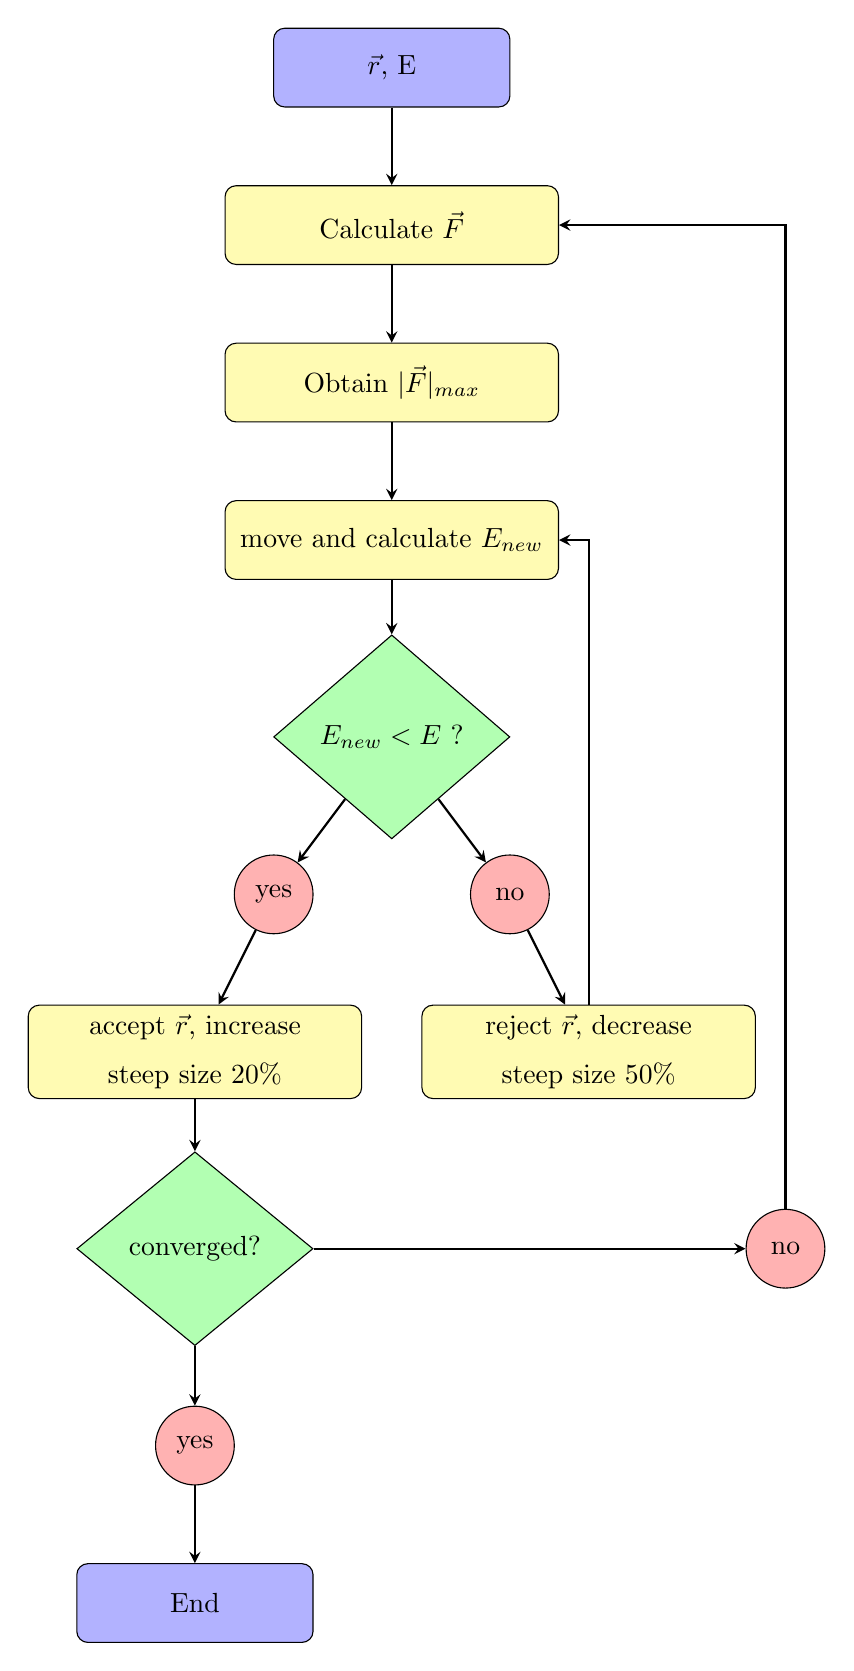
\begin{tikzpicture}[node distance=2cm]
      \node (start) [startstop] {$\vec{r}$, E};
      \node (forces) [element, below of=start ] {Calculate $\vec{F}$};
      \node (fmax) [element, below of=forces ] {Obtain  $|\vec{F}|_{max}$};
      \node (Enew) [element, below of=fmax ] {move and calculate $E_{new}$};
      \node (Edescend) [decision, below of=Enew, yshift=-0.5cm ] {$E_{new} < E$ ?};
      \node (yes2) [yes, below of=Edescend, xshift=-1.5cm ] {yes};
      \node (no2) [no, below of=Edescend, xshift=1.5cm ] {no};
      \node (increase) [element, below of=yes2, xshift=-1.0cm ] {accept $\vec{r}$, increase steep size 20\%};
      \node (decrease) [element, below of=no2, xshift=1.0cm ] {reject $\vec{r}$, decrease steep size 50\%};
      \node (converge) [decision, below of=increase, yshift=-0.5cm ] {converged?};
      \node (yes1) [yes, below of=converge, yshift=-0.5cm ] {yes};
      \node (no1) [no, right of=converge, xshift=5.5cm ] {no};
      \node (finish) [startstop, below of=yes1 ] {End};

      \draw [arrow] (start) -- (forces);
      \draw [arrow] (forces) -- (fmax);
      \draw [arrow] (fmax) -- (Enew);
      \draw [arrow] (Enew) -- (Edescend);
      \draw [arrow] (Edescend) -- (yes2);
      \draw [arrow] (Edescend) -- (no2);
      \draw [arrow] (yes2) -- (increase);
      \draw [arrow] (increase) -- (converge);
      \draw [arrow] (no2) -- (decrease);
      \draw [arrow] (decrease) |- (Enew);
      \draw [arrow] (converge) -- (yes1);
      \draw [arrow] (converge) -- (no1);
      \draw [arrow] (yes1) -- (finish);
      \draw [arrow] (no1) |- (forces);
    \end{tikzpicture}
    
    &

    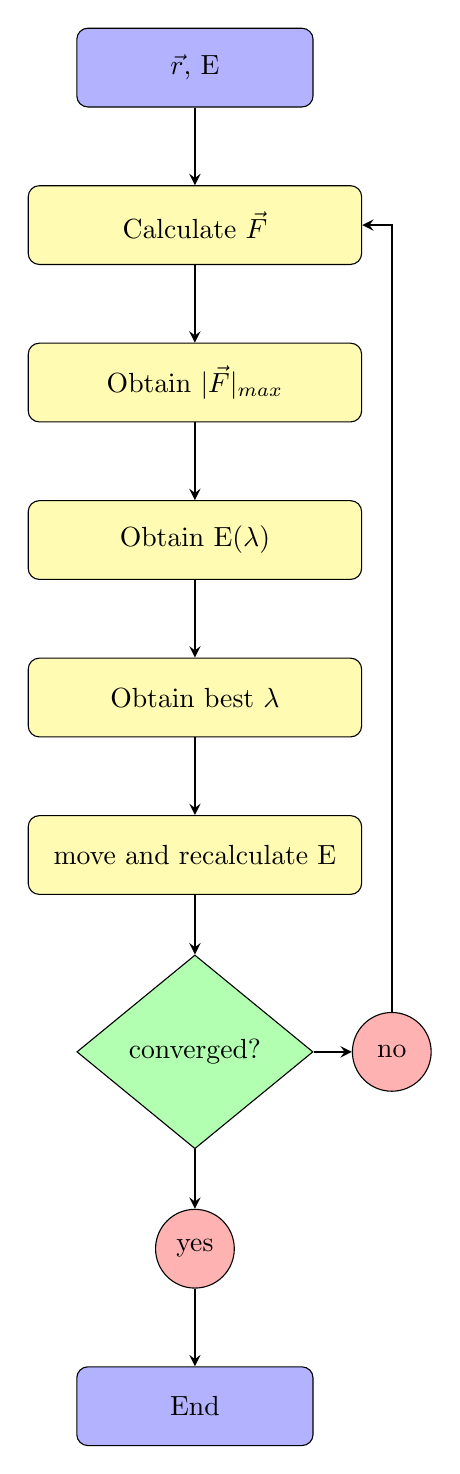
\begin{tikzpicture}[node distance=2cm]
      \node (start) [startstop] {$\vec{r}$, E};
      \node (forces) [element, below of=start ] {Calculate $\vec{F}$};
      \node (fmax) [element, below of=forces ] {Obtain  $|\vec{F}|_{max}$};
      \node (Elamb) [element, below of=fmax ] {Obtain  E($\lambda$)};
      \node (lamb) [element, below of=Elamb ] {Obtain best $\lambda$};
      \node (newr) [element, below of=lamb ] {move and recalculate E};
      \node (converge) [decision, below of=newr, yshift=-0.5cm ] {converged?};
      \node (yes1) [yes, below of=converge, yshift=-0.5cm ] {yes};
      \node (no1) [no, right of=converge, xshift=0.5cm ] {no};
      \node (finish) [startstop, below of=yes1 ] {End};

      \draw [arrow] (start) -- (forces);
      \draw [arrow] (forces) -- (fmax);
      \draw [arrow] (fmax) -- (Elamb);
      \draw [arrow] (Elamb) -- (lamb);
      \draw [arrow] (lamb) -- (newr);
      \draw [arrow] (newr) -- (converge);
      \draw [arrow] (converge) -- (yes1);
      \draw [arrow] (converge) -- (no1);
      \draw [arrow] (yes1) -- (finish);
      \draw [arrow] (no1) |- (forces);
    \end{tikzpicture}

       \end{tabular}
       \end{center}
      \label{steep-algorithm}
    \end{table}   
    
Best $\lambda$ in lineal search algorithm is obtained by a quadratic function ajusted using minimum energy of the scan and previous and next points.

    \subsection{Using geometry optimizations}
    
    Adding steep=t in LIO input enables geometry optimization (steepest descent, lineal search by default).
    Convergence criteria are set by Force\_cut and Energy\_cut (5E-4 Hartree/bohr and 1E-4 Hartree by Default).
    The number of minimization steeps is set by n\_min\_steps (500 by default) and initial distance steep is set by minimzation\_steep (by default 0.05 bohr)\\
    It is highly advisable to compile LIO in double precision in order to minimise the error in exchange-correlation forces (precision=1).
        Outputs of geometry optimizations are traj.xyz (atoms coordinates in each steepes descent movement) and optimization.out (steep, energy and others). If verbose=true optimization.out includes the energy of each linear search point.
    
    \subsection{Examples}
    
    Examples of geometry optimization are made in lio/test/13\_geom\_optim.
    
\newpage
\section{Restraints}
LIO may add an extra potential term to the Hamiltonian in order to restrain the distance between specified pairs of atoms.

    \subsection{Implemenation}
    The implementation is a simple harmonic potential over a generalized coordinate $r$.

    \begin{equation}
      U=\frac{1}{2} k [r - l_0]^2  
      \label{E_restrain}
    \end{equation}

    $r$ may be defined as a weighted combination of distances between pairs of atoms.

    \begin{equation}
      r=  \sum_{i} \sum_{j>i} w_{ij} |\vec{r_i} - \vec{r_j}|
      \label{gen_coord}
    \end{equation}

    In this formulation the force over an atom l is:

    \begin{equation}
      \vec{F_l}= -k [r - l_0] \sum_{i} \sum_{j>i} w_{ij} \frac{\vec{r_{ij}}}{r_{ij}} \eta_{ijl}     
      \label{rest_force}
    \end{equation}

    Where $\eta_{ijl}$ is defined as:

    \begin{equation*}
      \eta_{ijl} =
       \begin{cases}
          1 & \text{if $l=i$}\\
         -1 & \text{if $l=j$}\\
          0 & \text{in other case}
       \end{cases}
       \label{eta}
    \end{equation*}


    \subsection{Using Restraints}

    The number of pairs of atoms to be added in the restraint potential(s) is defined by setting the variable number\_restr, and a list of distance restrains have to be added to in an additional lio.restrain file. For example:

    \begin{table}  [H]
      \begin{center}
      \begin{tabular}{ l c c c c c}
         $a_i$ & $a_j$ & index &   k  &    $w_{ij}$   &  $l_0$    \\
         1  &  2 &   0   &  0.1 &    1.0   & 7.86   \\
         3  &  4 &   0   &  0.1 &   -1.0   & 7.86   \\
         7  &  9 &   1   &  0.4 &    2.0   & -2.3   \\
         13 &  1 &   1   &  0.4 &    1.0   & -2.3   \\
         14 &  3 &   1   &  0.4 &   -3.0   & -2.3   \\
         14 &  2 &   2   &  0.2 &    1.0   & 0.5    \\
         8  &  5 &   3   &  0.3 &    1.0   & 3.2    \\
       \end{tabular}
       \end{center}
      \label{lio.restrain}
    \end{table}

Columns $a_i$ and $a_j$ contain the atom numbers in the QM system to be restrained, while the index number determines which distances contribute to a same generalized reaction coordinate. The remaining columns are the force constants (k), weights of that distance in the generalized coordinate ($w_{ij}$) and equilibrium positions in atomic units ($l_0$).

    \subsection{Examples}

    \textbf{1)In lio.in:}
    
    number\_restr = 1
    
        \textbf{in lio.restrain:}

    \begin{table}  [H]
      \begin{center}
      \begin{tabular}{ l c c c c c}
         $a_i$ & $a_j$ & index &   k  &    $w_{ij}$   &  $l_0$   \\
         1  &  2 &   0   &  0.1 &    1.0   & 7.86   \\
       \end{tabular}
       \end{center}
      \label{Tex1}
    \end{table}

    \textbf{Potential added to system:}

    \begin{equation}
      U=\frac{1}{2} 0.1 \Big{[} 1.0 |\vec{r_1} - \vec{r_2}| - 7.86\Big{]}^2  
      \label{Ex1}
    \end{equation}


    \textbf{2)In lio.in:}

    number\_restr = 2

    \textbf{in lio.restrain:}

    \begin{table}  [H]
      \begin{center}
      \begin{tabular}{ l c c c c c}
         $a_i$ & $a_j$ & index &   k  &    $w_{ij}$   &  $l_0$    \\
         1  &  2 &   0   &  0.1 &    1.0   & 7.86   \\
         3  &  4 &   0   &  0.1 &   -1.0   & 7.86   \\
       \end{tabular}
       \end{center}
      \label{Tex2}
    \end{table}

    \textbf{Potential added to system:}

    \begin{equation}
      U=\frac{1}{2} 0.1 \Big{[} 1.0 |\vec{r_1} - \vec{r_2}| - 1.0 |\vec{r_3} - \vec{r_4}| - 7.86\Big{]}^2  
      \label{Ex2}
    \end{equation}


    \textbf{3)In lio.in:}

    number\_restr = 4

    \textbf{in lio.restrain:}

    \begin{table}  [H]
      \begin{center}
      \begin{tabular}{ l c c c c c}
         $a_i$ & $a_j$ & index &   k  &    $w_{ij}$   &  $l_0$    \\
         1  &  2 &   0   &  0.1 &    1.0   & 7.86   \\
         3  &  4 &   0   &  0.1 &   -1.0   & 7.86   \\
         1  &  3 &   1   &  0.3 &    3.5   & -2.31   \\
         7  &  8 &   1   &  0.3 &   -2.2   & -2.31   \\
       \end{tabular}
       \end{center}
      \label{Tex3}
    \end{table}

    \textbf{Potential added to system:}

    \begin{equation}
      U=\frac{1}{2} 0.1 \Big{[} 1.0 |\vec{r_1} - \vec{r_2}| - 1.0 |\vec{r_3} - \vec{r_4}| - 7.86\Big{]}^2 + \frac{1}{2} 0.3 \Big{[} 3.5 |\vec{r_1} - \vec{r_3}| - 2.2 |\vec{r_7} - \vec{r_8}| +2.31\Big{]}^2 
      \label{Ex3}
    \end{equation}



%\addtocontents{toc}{\protect\newpage}
\chapter{Electron Dynamics}

\section{Real Time TD-DFT}

\section{Electronic transport}

\section{Ehrenfest Dynamics}



%\addtocontents{toc}{\protect\newpage}
\chapter{Post-Processing Tools}

\section{TD-Analize: Electronic Spectra}

\section{CubeGen: Orbital and Density Visualization}



%\addtocontents{toc}{\protect\newpage}
%%%%%%%%%%%%%%%%%%%%%%%%%%%%%%%%%%%%%%%%%%%%%%%%%%%%%%%%%%%%
\chapter{Reference Section}

This section contains a quick reference for all of LIO's input variables
and commandline options. For more detailed descriptions, please refer to 
the previous chapters.

%%%%%%%%%%%%%%%%%%%%%%%%%%%%%%%%%%%%%%%%%%%%%%%%%%%%%%%%%%%%
\section{Command line options}

%%%%%%%%%%%%%%%%%%%%%%%%%%%%%%%%%%%%%%%%%%%%%%%%%%%%%%%%%%%%
\begin{Spacing}{1.0}
   \begin{longtable}{ p{.25\textwidth} p{.70\textwidth} }
   
      \toprule
      \textbf{Variable} & Description \\*
      \midrule \\*
      \endhead
   
      \bottomrule
      \caption{Command Line}
      \endfoot

      \textbf{-i file\_name}
      &  \textit{default = 'lio.in' }
      \\*\textit{character*20}
      & Name of the input file containing LIO options. \\* \\

      \textbf{-c crd\_file.xyz}
      &  \textit{default = 'qm.xyz' }
      \\*\textit{character*20}
      & Name of thte XYZ file containing coordinates. \\* \\
      
      \textbf{-b basis\_file}
      &  \textit{default = 'basis' }
      \\*\textit{character*20}
      & A file containing the basis set and fitting set data,
      only used when int\_basis=f. \\* \\

      \textbf{-v}
      &  \textit{default = .false. }
      \\*\textit{logical}
      & Sets verbose level to 4.\\* \\
   
   
   \end{longtable}
\end{Spacing}
%%%%%%%%%%%%%%%%%%%%%%%%%%%%%%%%%%%%%%%%%%%%%%%%%%%%%%%%%%%%
   
\newpage

%%%%%%%%%%%%%%%%%%%%%%%%%%%%%%%%%%%%%%%%%%%%%%%%%%%%%%%%%%%%
\section{Keywords - General Setup}

%%%%%%%%%%%%%%%%%%%%%%%%%%%%%%%%%%%%%%%%%%%%%%%%%%%%%%%%%%%%
\begin{Spacing}{1.0}
\begin{longtable}{ p{.25\textwidth} p{.70\textwidth} }

   \toprule
   \textbf{Variable} & Description \\*
   \midrule \\*
   \endhead

   \bottomrule
   \caption{General Setup}
   \endfoot

   \textbf{natom}
   &  \textit{default = 0 }
   \\*\textit{integer}
   & Number of QM atoms in the system.\\* \\

   \textbf{nsol}
   &  \textit{default = 0 }
   \\*\textit{integer}
   & Number of classical atoms in the system.\\* \\

   \textbf{charge}
   &  \textit{default = 0 }
   \\*\textit{integer}
   & Total charge of the QM system.\\* \\

   \textbf{open}
   &  \textit{default = .false. }
   \\*\textit{logical}
   & Perform an open-shell calculation.\\* \\

   \textbf{nunp}
   &  \textit{default = 0 }
   \\*\textit{integer}
   & Number of unpaired electrons for open-shell
   calculations.\\* \\

   \textbf{style}
   &  \textit{default = .false. }
   \\*\textit{logical}
   & Activates a formatted version of the output.\\* \\

   \textbf{fcoord}
   &  \textit{default = 'qm.xyz' }
   \\*\textit{character*20}
   & Name of the output file for the coordinates of the
   QM system.\\* \\

   \textbf{writexyz}
   &  \textit{default = .false. }
   \\*\textit{logical}
   & Writes an xyz file containing the QM system.\\* \\

   \textbf{verbose}
   &  \textit{default = 1 }
   \\*\textit{integer}
   & Determines the amount of information printed, from 
   0 (nothing) to 5 (everything). \\* \\

   \textbf{timers}
   &  \textit{default = 0}
   \\*\textit{integer}
   & Activates timers (=1 or =2).\\* \\

   \textbf{dbug}
   &  \textit{default = .false. }
   \\*\textit{logical}
   & Checks for NaNs. \\* \\

    \textbf{writeForces}
   &  \textit{default = .false. }
   \\*\textit{logical}
   & Writes final forces to an output file.\\* \\

   \textbf{dipole}
   &  \textit{default = .false. }
   \\*\textit{logical}
   & Calculates and prints dipole moment.\\* \\

   \textbf{mulliken}
   &  \textit{default = .false. }
   \\*\textit{logical}
   & Performs a Mulliken Population Analysis.\\* \\

   \textbf{lowdin}
   &  \textit{default = .false. }
   \\*\textit{logical}
   & Performs a Lowdin Population Analysis.\\* \\

   \textbf{fukui}
   &  \textit{default = .false. }
   \\*\textit{logical}
   & Calculates atomic Fukui function.\\* \\

   \textbf{gaussian\_convert}
   &  \textit{default = .false. }
   \\*\textit{logical}
   & Reads a Gaussian09 density matrix.\\* \\

   \textbf{print\_coeffs}
   &  \textit{default = .false. }
   \\*\textit{logical}
   & Prints MO coefficients in AO basis.\\* \\

\end{longtable}
\end{Spacing}
%%%%%%%%%%%%%%%%%%%%%%%%%%%%%%%%%%%%%%%%%%%%%%%%%%%%%%%%%%%%

\newpage
%%%%%%%%%%%%%%%%%%%%%%%%%%%%%%%%%%%%%%%%%%%%%%%%%%%%%%%%%%%%
\section{Keywords - GPU Options}

%%%%%%%%%%%%%%%%%%%%%%%%%%%%%%%%%%%%%%%%%%%%%%%%%%%%%%%%%%%%
\begin{Spacing}{1.0}
\begin{longtable}{ p{.35\textwidth} p{.60\textwidth} }

   \toprule
   \textbf{Variable} & Description \\*
   \midrule \\*
   \endhead

   \bottomrule
   \caption{GPU Module Options}
   \endfoot

   \textbf{gpu\_level}
   &  \textit{default = 4}
   \\*\textit{integer}
   & Determines which calculations are performed by
   the GPU. (0 = only XC, 5 = everything).\\*\\

   \textbf{max\_function\_exponent}
   &  \textit{default = 10}
   \\*\textit{integer}
   & Ignore functions with $\lvert exponent \rvert > 
   max\_function\_exponent$.\\* \\

   \textbf{little\_cube\_size}
   &  \textit{default = 8.0d0}
   \\*\textit{double precision}
   & Small cube-type point group size.\\* \\

   \textbf{min\_points\_per\_cube}
   &  \textit{default = 1}
   \\*\textit{integer}
   & Minimum number of grid points in a cube.\\* \\

   \textbf{assign\_all\_functions}
   &  \textit{default = .false. }
   \\*\textit{logical}
   & Calculate all functions (ignores
   $max\_function\_exponent$).\\* \\

   \textbf{sphere\_radius}
   &  \textit{default = 0.6d0}
   \\*\textit{double precision}
   & Proportion of points contained in sphere-type groups (from 0 to 1).\\* \\

   \textbf{remove\_zero\_weights}
   &  \textit{default = .true. }
   \\*\textit{logical}
   & Discard functions for those whose weight is zero.
   \\* \\

   \textbf{energy\_all\_iterations}
   &  \textit{default = .false. }
   \\*\textit{logical}
   & Calculate Exc energy in all SCF iterations.\\* \\

   \textbf{free\_global\_memory}
   &  \textit{default = 0.0d0}
   \\*\textit{double precision}
   & Fraction of global GPU memory available for the
   calculation (1 means 100\%).\\* \\

\end{longtable}
\end{Spacing}
%%%%%%%%%%%%%%%%%%%%%%%%%%%%%%%%%%%%%%%%%%%%%%%%%%%%%%%%%%%%

\newpage
%%%%%%%%%%%%%%%%%%%%%%%%%%%%%%%%%%%%%%%%%%%%%%%%%%%%%%%%%%%%
\section{Keywords - DFT Hamiltonian}

%%%%%%%%%%%%%%%%%%%%%%%%%%%%%%%%%%%%%%%%%%%%%%%%%%%%%%%%%%%%
\begin{Spacing}{1.0}
\begin{longtable}{ p{.25\textwidth} p{.70\textwidth} }

   \toprule
   \textbf{Variable} & Description \\*
   \midrule \\*
   \endhead

   \bottomrule
   \caption{DFT Hamiltonian}
   \endfoot

   \textbf{iexch}
   &  \textit{default = 9}
   \\*\textit{integer}
   & Identifies the exchange-correlation potential to use
   with the calculation when not using libxc.\\*
   & Iexch=9 is the only option currently available.\\* \\

   \textbf{use\_libxc}
   &  \textit{default = .false. }
   \\*\textit{logical}
   & Activates the use of libxc version of the XC
   potential.\\* \\

   \textbf{ex\_functional\_id}
   &  \textit{default = ?}
   \\*\textit{integer}
   & Exchange functional to use with libxc.\\* \\

   \textbf{ec\_functional\_id}
   &  \textit{default = ?}
   \\*\textit{integer}
   & Correlation functional to use with libxc.\\* \\

   \textbf{int\_basis}
   &  \textit{default = .true. }
   \\*\textit{logical}
   & If true, looks for the internal basis indicated in
   variables $basis\_set$ and $fitting\_set$; if false, 
   an external basis file must be provided. \\* \\

   \textbf{basis\_set}
   &  \textit{default = 'DZVP'}
   \\*\textit{character*20}
   & Name of the basis set used, or the name of the
   custom basis set file.\\* \\

   \textbf{fitting\_set}
   &  \textit{default = 'DZVP Coulomb Fitting'}
   \\*\textit{character*100}
   & Name of the fitting set used in the calculation.\\* \\

   \textbf{n\_ghosts}
   &  \textit{default = 0}
   \\*\textit{integer}
   & Number of ghost atoms.\\* \\

   \textbf{ghost\_atoms}
   &  \textit{default = 0}
   \\*\textit{integer}
   & A list containing the ghost atom indeces. \\* \\

   \textbf{rmax}
   &  \textit{default = 16.0d0}
   \\*\textit{double precision}
   & Maximum exponent in 3-center integrals.
   \\* \\

   \textbf{rmaxs}
   &  \textit{default = 5.0d0}
   \\*\textit{double precision}
   & Maximum exponent for 3-center integrals in single
   precision.\\* \\

   \textbf{iGrid}
   &  \textit{default = 2}
   \\*\textit{integer}
   & Grid type when iterating through SCF.\\* \\

   \textbf{iGrid2}
   &  \textit{default = 2}
   \\*\textit{integer}
   & Grid type for final energy calculation in SCF.\\* \\


\end{longtable}
\end{Spacing}
%%%%%%%%%%%%%%%%%%%%%%%%%%%%%%%%%%%%%%%%%%%%%%%%%%%%%%%%%%%%

\newpage
%%%%%%%%%%%%%%%%%%%%%%%%%%%%%%%%%%%%%%%%%%%%%%%%%%%%%%%%%%%%
\section{Keywords - Effective Core Potentials}

%%%%%%%%%%%%%%%%%%%%%%%%%%%%%%%%%%%%%%%%%%%%%%%%%%%%%%%%%%%%
\begin{Spacing}{1.0}
\begin{longtable}{ p{.25\textwidth} p{.70\textwidth} }

   \toprule
   \textbf{Variable} & Description \\*
   \midrule \\*
   \endhead

   \bottomrule
   \caption{Effective Core Potentials}
   \endfoot

   \textbf{ECPMode}
   &  \textit{default = .false. }
   \\*\textit{logical}
   & Activate effective core potentials.\\* \\

   \textbf{ECPTypes}
   &  \textit{default = 0}
   \\*\textit{integer}
   & Number of atoms with ECP.\\* \\

   \textbf{tipeECP}
   &  \textit{default = 'NOT-DEFINED'}
   \\*\textit{character*30}
   & Type of ECP used.\\* \\

   \textbf{ZListECP}
   &  \textit{default = 0}
   \\*\textit{integer}
   & Array with Z of atoms with ECP enabled.\\* \\

   \textbf{cutECP}
   &  \textit{default = .true. }
   \\*\textit{logical}
   & Enables cuts for ECP integrals.\\* \\

   \textbf{cut2\_0}
   &  \textit{default = 15.d0}
   \\*\textit{double precision}
   & Cut value for 2-center ECP integrals.\\* \\

   \textbf{cut3\_0}
   &  \textit{default = 12.d0}
   \\*\textit{double precision}
   & Cut value for 3-center ECP integrals.\\* \\

   \textbf{ECP\_debug}
   &  \textit{default = .false. }
   \\*\textit{logical}
   & Enables ECP debug mode.\\* \\

   \textbf{local\_nonlocal}
   &  \textit{default = 0}
   \\*\textit{integer}
   & Calculates only local terms (when = 1) or
   only non-local terms (when = 2).\\* \\

   \textbf{ECP\_full\_range\_int}
   &  \textit{default = .false. }
   \\*\textit{logical}
   & Enables full-range integral calculations.\\* \\

   \textbf{verbose\_ECP}
   &  \textit{default = 0}
   \\*\textit{integer}
   & Controls ECP verbose levels.\\* \\

   \textbf{fock\_ECP\_read}
   &  \textit{default = .false. }
   \\*\textit{logical}
   & Enables restart read in ECP.\\* \\

   \textbf{fock\_ECP\_write}
   &  \textit{default = .false. }
   \\*\textit{logical}
   & Enables restart write in ECP.\\* \\

   \textbf{fullTimer\_ECP}
   &  \textit{default = .false. }
   \\*\textit{logical}
   & Enables full timers in ECP.\\* \\

\end{longtable}
\label{tablaECP2}
\end{Spacing}
%%%%%%%%%%%%%%%%%%%%%%%%%%%%%%%%%%%%%%%%%%%%%%%%%%%%%%%%%%%%

\newpage
%%%%%%%%%%%%%%%%%%%%%%%%%%%%%%%%%%%%%%%%%%%%%%%%%%%%%%%%%%%%
\section{Keywords - DFTB Embedding}

%%%%%%%%%%%%%%%%%%%%%%%%%%%%%%%%%%%%%%%%%%%%%%%%%%%%%%%%%%%%
\begin{Spacing}{1.0}
\begin{longtable}{ p{.25\textwidth} p{.70\textwidth} }

   \toprule
   \textbf{Variable} & Description \\*
   \midrule \\*
   \endhead

   \bottomrule
   \caption{DFTB Embedding}
   \endfoot

   \textbf{dftb\_calc}
   &  \textit{default = .false. }
   \\*\textit{logical}
   & Activates the TB embedding of the system.\\* \\

   \textbf{MTB}
   &  \textit{default = 0}
   \\*\textit{integer}
   & TODO Size of the two tight-binding subatrices.\\* \\

   \textbf{end\_bTB}
   &  \textit{default = 0}
   \\*\textit{integer}
   & TODO Index matrix size.\\* \\

   \textbf{start\_tdtb}
   &  \textit{default = 0}
   \\*\textit{integer}
   & TODO Initial time step for evolution of diagonal TB 
   terms (????).\\* \\

   \textbf{end\_tdtb}
   &  \textit{default = 0}
   \\*\textit{integer}
   & TODO Final time step for evolution of diagonal TB
   terms (????).\\* \\

   \textbf{alfaTB}
   &  \textit{default = UNSET}
   \\*\textit{double precision}
   & Manually sets the on-site energies (diagonal values)
   for the TB part of the Hamiltonian.\\* \\

   \textbf{betaTB}
   &  \textit{default = UNSET}
   \\*\textit{double precision}
   & Manually sets the hopping terms for the TB part of
   the Hamiltonian (ie, the non-diagonal nearest neighbour
   terms for TB - TB interactions).\\* \\

   \textbf{gammaTB}
   &  \textit{default = UNSET}
   \\*\textit{double precision}
   & Manually sets the hopping terms for the interaction
   between TB atoms and DFT atoms.\\* \\

   \textbf{Vbias\_TB}
   &  \textit{default = UNSET}
   \\*\textit{double precision}
   & Sets a bias for the on-site energies to simulate
   electrodes.\\* \\

   \textbf{TBload}
   &  \textit{default = .false. }
   \\*\textit{logical}
   & TODO.\\* \\

   \textbf{TBsave}
   &  \textit{default = .false. }
   \\*\textit{logical}
   & TODO.\\* \\

\end{longtable}
\end{Spacing}
%%%%%%%%%%%%%%%%%%%%%%%%%%%%%%%%%%%%%%%%%%%%%%%%%%%%%%%%%%%%

\newpage
%%%%%%%%%%%%%%%%%%%%%%%%%%%%%%%%%%%%%%%%%%%%%%%%%%%%%%%%%%%%
\section{Keywords - Fields and Biases}

%%%%%%%%%%%%%%%%%%%%%%%%%%%%%%%%%%%%%%%%%%%%%%%%%%%%%%%%%%%%
\begin{Spacing}{1.0}
\begin{longtable}{ p{.25\textwidth} p{.70\textwidth} }

   \toprule
   \textbf{Variable} & Description \\*
   \midrule \\*
   \endhead

   \bottomrule
   \caption{Fields and Biases}
   \endfoot

   \textbf{field}
   &  \textit{default = .false. }
   \\*\textit{logical}
   & Use an external field (perturbation in TD).\\* \\

   \textbf{a0}
   &  \textit{default = 1.0d3}
   \\*\textit{double precision}
   & A dividing factor in electric field calculations.\\* \\

   \textbf{epsilon}
   &  \textit{default = 1.0d0}
   \\*\textit{double precision}
   & Relative permitivity of the medium.\\* \\

   \textbf{Fx, Fy, Fz}
   &  \textit{default = 0.05d0}
   \\*\textit{double precision}
   & The value of the external electric field in the
   x, y and z directions.\\* \\

   \textbf{nfields\_iso}
   &  \textit{default = 0}
   \\*\textit{integer}
   & Number of shape-isotropic fields. \\* \\

   \textbf{field\_iso\_file}
   &  \textit{default = 'field.in'}
   \\*\textit{character*20}
   & Isotropic fields input file.\\* \\

   \textbf{nfields\_aniso}
   &  \textit{default = 0}
   \\*\textit{integer}
   & Number of shape-anisotropic fields. \\* \\

   \textbf{field\_aniso\_file}
   &  \textit{default = 'field.in'}
   \\*\textit{character*20}
   & Anisotropic fields input file.\\* \\

   \textbf{fockbias\_is\_active}
   &  \textit{default = .false. }
   \\*\textit{logical}
   & TODO.\\* \\

   \textbf{fockbias\_is\_shaped}
   &  \textit{default = .false. }
   \\*\textit{logical}
   & TODO.\\* \\

   \textbf{fockbias\_readfile}
   &  \textit{default = 'atombias.in'}
   \\*\textit{character*80}
   & Atomic bias input file.\\* \\

   \textbf{fockbias\_timeamp0}
   &  \textit{default = UNSET}
   \\*\textit{double precision}
   & TODO.\\* \\

   \textbf{fockbias\_timefall}
   &  \textit{default = UNSET}
   \\*\textit{double precision}
   & TODO.\\* \\

   \textbf{fockbias\_timegrow}
   &  \textit{default = UNSET}
   \\*\textit{double precision}
   & TODO.\\* \\

\end{longtable}
\end{Spacing}
%%%%%%%%%%%%%%%%%%%%%%%%%%%%%%%%%%%%%%%%%%%%%%%%%%%%%%%%%%%%

\newpage
%%%%%%%%%%%%%%%%%%%%%%%%%%%%%%%%%%%%%%%%%%%%%%%%%%%%%%%%%%%%
\section{Keywords - Self Consistent Field}

%%%%%%%%%%%%%%%%%%%%%%%%%%%%%%%%%%%%%%%%%%%%%%%%%%%%%%%%%%%%
\begin{Spacing}{1.0}
\begin{longtable}{ p{.25\textwidth} p{.70\textwidth} }

   \toprule
   \textbf{Variable} & Description \\*
   \midrule \\*
   \endhead

   \bottomrule
   \caption{Self Consistent Field}
   \endfoot

   \textbf{initial\_guess}
   &  \textit{default = 0}
   \\*\textit{integer}
   & Method for generating the initial guess for the
   SCF.\\* \\

   \textbf{nMax}
   &  \textit{default = 100}
   \\*\textit{integer}
   & Maximum number of SCF steps.\\* \\

   \textbf{told}
   &  \textit{default = 1.0d-6}
   \\*\textit{double precision}
   & Tolerance threshold for density matrix convergence.\\* \\

   \textbf{Etold}
   &  \textit{default = 1.0d0}
   \\*\textit{double precision}
   & Tolerance threshold for energy convergence.\\* \\

   \textbf{DIIS}
   &  \textit{default = .true. }
   \\*\textit{logical}
   & Use DIIS convergence accelerator if true, or damping
   convergence accelerator if false.\\* \\

   \textbf{nDIIS}
   &  \textit{default = 30}
   \\*\textit{integer}
   & Number of DIIS convergence iterations.\\* \\

   \textbf{gold}
   &  \textit{default = 1.0d1}
   \\*\textit{double precision}
   & Proportion of old matrix to use when using the damping
   mixture (gold = X means that it will use an 1:X new to
   old proportion).\\* \\

   \textbf{hybrid\_converg}
   &  \textit{default = .false. }
   \\*\textit{logical}
   & Use Hybrid convergence accelerator.\\* \\

   \textbf{good\_cut}
   &  \textit{default = 1.0d-5}
   \\*\textit{double precision}
   & Tolerance threshold for damped convergence, switch to
   DIIS afterwards.\\* \\

   \textbf{vcinp}
   &  \textit{default = .false. }
   \\*\textit{logical}
   & Reads the molecular orbital coefficients from $frestart$
   and uses that as the starting guess for the first SCF
   cycle.\\* \\

   \textbf{rst\_dens}
   &  \textit{default = 0}
   \\*\textit{integer}
   & rst\_dens = 1 reads a density matrix restart, while rst\_dens = 2
        both reads and writes a density matrix restart. \\
   \\

   \textbf{frestartin}
   &  \textit{default = 'restart.in'}
   \\*\textit{character*20}
   & Filename for the input containing the molecular orbital
   coefficients to be used as starting guess when $vcinp =
   .true.$.\\* \\

   \textbf{frestart}
   &  \textit{default = 'restart.out'}
   \\*\textit{character*20}
   & Filename for the output containing the molecular orbital 
   coefficients.\\* \\

   \textbf{restart\_freq}
   &  \textit{default = 0}
   \\*\textit{integer}
   & Indicates the frequency for writing the restart: it will
   do so every set number of calls to LIO (that is, number of
   steps of nuclear moves performed by the MD-engine.\\* \\

\end{longtable}
\end{Spacing}
%%%%%%%%%%%%%%%%%%%%%%%%%%%%%%%%%%%%%%%%%%%%%%%%%%%%%%%%%%%%

\newpage
%%%%%%%%%%%%%%%%%%%%%%%%%%%%%%%%%%%%%%%%%%%%%%%%%%%%%%%%%%%%
\section{Keywords - Geometry Optimization}

%%%%%%%%%%%%%%%%%%%%%%%%%%%%%%%%%%%%%%%%%%%%%%%%%%%%%%%%%%%%
\begin{Spacing}{1.0}
\begin{longtable}{ p{.25\textwidth} p{.70\textwidth} }

   \toprule
   \textbf{Variable} & Description \\*
   \midrule \\*
   \endhead

   \bottomrule
   \caption{Geometry Optimization}
   \endfoot

   \textbf{steep}
   &  \textit{default = .false. }
   \\*\textit{logical}
   & Activate steepest descent algorithm for geometry
   optimization.\\* \\

   \textbf{Force\_cut}
   &  \textit{default = 5.0d-4}
   \\*\textit{double precision}
   & Convergence criteria in forces (Hartree/bohr) for
   geometry optimization.\\* \\

   \textbf{Energy\_cut}
   &  \textit{default = 1.0d-4}
   \\*\textit{double precision}
   & Convergence criteria in energy (Hartree) for 
   geometry optimization.\\* \\

   \textbf{minimzation\_steep}
   &  \textit{default = 0.05d0}
   \\*\textit{double precision}
   & Initial distance steep (bohr).\\* \\

   \textbf{n\_min\_steeps}
   &  \textit{default = 500}
   \\*\textit{integer}
   & Maximum number of geometry optimization steps.\\* \\

   \textbf{lineal\_search}
   &  \textit{default = .true. }
   \\*\textit{logical}
   & Enable lineal search algorithm.\\* \\

   \textbf{n\_points}
   &  \textit{default = 5}
   \\*\textit{integer}
   & Number of points scaned for lineal search.\\* \\

   \textbf{number\_restr}
   &  \textit{default = 0}
   \\*\textit{integer}
   & Number of distance restraints used.\\* \\


\end{longtable}
\end{Spacing}
%%%%%%%%%%%%%%%%%%%%%%%%%%%%%%%%%%%%%%%%%%%%%%%%%%%%%%%%%%%%

\newpage
%%%%%%%%%%%%%%%%%%%%%%%%%%%%%%%%%%%%%%%%%%%%%%%%%%%%%%%%%%%%
\section{Keywords - Real Time TD-DFT}

%%%%%%%%%%%%%%%%%%%%%%%%%%%%%%%%%%%%%%%%%%%%%%%%%%%%%%%%%%%%
\begin{Spacing}{1.0}
\begin{longtable}{ p{.25\textwidth} p{.70\textwidth} }

   \toprule
   \textbf{Variable} & Description \\*
   \midrule \\*
   \endhead

   \bottomrule
   \caption{Real Time TD-DFT}
   \endfoot

   \textbf{timeDep}
   &  \textit{default = 0}
   \\*\textit{integer}
   & Use RT-TD-DFT when timeDep = 1.\\* \\

   \textbf{tdStep}
   &  \textit{default = 2.0d-5}
   \\*\textit{double precision}
   & Timestep for TD-DFT (in atomic units).\\* \\

   \textbf{ntdStep}
   &  \textit{default = 0}
   \\*\textit{integer}
   & Total number of TD-DFT steps.\\* \\

   \textbf{propagator}
   &  \textit{default = 1}
   \\*\textit{integer}
   & RT-TD-DFT propagator (1 = Verlet, 2 = Magnus).\\* \\

   \textbf{NBCH}
   &  \textit{default = 10}
   \\*\textit{integer}
   & Number of [$\rho$. Fock\textsuperscript{n}] commutators
   in Magnus.\\* \\

   \textbf{tdrestart}
   &  \textit{default = .false. }
   \\*\textit{logical}
   & Reads an input restart for TD ( named td\_in.restart ).\\* \\

   \textbf{td\_rst\_freq}
   &  \textit{default = 500}
   \\*\textit{integer}
   & Write the TD restart every $td\_rst\_freq$ steps.\\* \\

   \textbf{td\_do\_pop}
   &  \textit{default = 0}
   \\*\textit{integer}
   & Number of step stride in which the pop will be written.
   (0 means it is never written).\\* \\


\end{longtable}
\end{Spacing}
%%%%%%%%%%%%%%%%%%%%%%%%%%%%%%%%%%%%%%%%%%%%%%%%%%%%%%%%%%%%

\newpage
%%%%%%%%%%%%%%%%%%%%%%%%%%%%%%%%%%%%%%%%%%%%%%%%%%%%%%%%%%%%
\section{Keywords - Transport}

%%%%%%%%%%%%%%%%%%%%%%%%%%%%%%%%%%%%%%%%%%%%%%%%%%%%%%%%%%%%
\begin{Spacing}{1.0}
\begin{longtable}{ p{.25\textwidth} p{.70\textwidth} }

   \toprule
   \textbf{Variable} & Description \\*
   \midrule \\*
   \endhead

   \bottomrule
   \caption{Transport}
   \endfoot

   \textbf{transport\_calc}
   &  \textit{default = .false. }
   \\*\textit{logical}
   & TODO.\\* \\

   \textbf{generate\_rho0}
   &  \textit{default = .false. }
   \\*\textit{logical}
   & TODO.\\* \\

   \textbf{gate\_field}
   &  \textit{default = .false. }
   \\*\textit{logical}
   & TODO.\\* \\

   \textbf{driving\_rate}
   &  \textit{default = UNSET}
   \\*\textit{double precision}
   & TODO.\\* \\

   \textbf{pop\_drive}
   &  \textit{default = UNSET}
   \\*\textit{integer}
   & TODO.\\* \\

   \textbf{save\_charge\_freq}
   &  \textit{default = UNSET}
   \\*\textit{integer}
   & TODO.\\* \\

   \textbf{nbias}
   &  \textit{default = UNSET}
   \\*\textit{integer}
   & TODO.\\* \\

\end{longtable}
\end{Spacing}
%%%%%%%%%%%%%%%%%%%%%%%%%%%%%%%%%%%%%%%%%%%%%%%%%%%%%%%%%%%%

\newpage
%%%%%%%%%%%%%%%%%%%%%%%%%%%%%%%%%%%%%%%%%%%%%%%%%%%%%%%%%%%%
\section{Keywords - Ehrenfest}

%%%%%%%%%%%%%%%%%%%%%%%%%%%%%%%%%%%%%%%%%%%%%%%%%%%%%%%%%%%%
\begin{Spacing}{1.0}
\begin{longtable}{ p{.25\textwidth} p{.70\textwidth} }

   \toprule
   \textbf{Variable} & Description \\*
   \midrule \\*
   \endhead

   \bottomrule
   \caption{Ehrenfest}
   \endfoot

   \textbf{ndyn\_steps}
   &  \textit{default = 0}
   \\*\textit{integer}
   & Number of nuclear movement steps.\\* \\

   \textbf{rsto\_nfreq}
   &  \textit{default = 0}
   \\*\textit{integer}
   & Frequency (in steps) in which the restart is printed.
   (A value of 0 means only written in the end)\\* \\

   \textbf{rsto\_saves}
   &  \textit{default = .false. }
   \\*\textit{logical}
   & TODO.\\* \\

   \textbf{rsti\_loads}
   &  \textit{default = .false. }
   \\*\textit{logical}
   & TODO.\\* \\

   \textbf{nullify\_forces}
   &  \textit{default = .false. }
   \\*\textit{logical}
   & Returns 0 for all forces to the MD engine.\\* \\

   \textbf{nullify\_forces}
   &  \textit{default = .false. }
   \\*\textit{logical}
   & Returns 0 for all forces to the MD engine.\\* \\

   \textbf{eefld\_on}
   &  \textit{default = .false. }
   \\*\textit{logical}
   & TODO.\\* \\

   \textbf{eefld\_timegih}
   &  \textit{default = .false. }
   \\*\textit{logical}
   & TODO.\\* \\

   \textbf{eefld\_timegfh}
   &  \textit{default = .false. }
   \\*\textit{logical}
   & TODO.\\* \\

   \textbf{eefld\_ampx/ampy/ampz}
   &  \textit{default = 2.D-5}
   \\*\textit{double precision}
   & TODO.\\* \\

   \textbf{eefld\_timeamp}
   &  \textit{default = 2.D-5}
   \\*\textit{double precision}
   & TODO.\\* \\

   \textbf{eefld\_timepos}
   &  \textit{default = 2.D-5}
   \\*\textit{double precision}
   & TODO.\\* \\

   \textbf{eefld\_wavelen}
   &  \textit{default = 2.D-5}
   \\*\textit{double precision}
   & TODO.\\* \\


\end{longtable}
\end{Spacing}
%%%%%%%%%%%%%%%%%%%%%%%%%%%%%%%%%%%%%%%%%%%%%%%%%%%%%%%%%%%%

\newpage
%%%%%%%%%%%%%%%%%%%%%%%%%%%%%%%%%%%%%%%%%%%%%%%%%%%%%%%%%%%%
\section{Keywords - CubeGen}

%%%%%%%%%%%%%%%%%%%%%%%%%%%%%%%%%%%%%%%%%%%%%%%%%%%%%%%%%%%%
\begin{Spacing}{1.0}
\begin{longtable}{ p{.25\textwidth} p{.70\textwidth} }

   \toprule
   \textbf{Variable} & Description \\*
   \midrule \\*
   \endhead

   \bottomrule
   \caption{CubeGen}
   \endfoot

   \textbf{cube\_dens}
   &  \textit{default = .false. }
   \\*\textit{logical}
   & Prints the electronic density.\\* \\

   \textbf{cubeGen\_only}
   &  \textit{default = .false. }
   \\*\textit{logical}
   & Avoid running SCF, only do cubeGen from a restart.\\* \\

   \textbf{cube\_res}
   &  \textit{default = 40}
   \\*\textit{integer}
   & Number of voxels per dimension (resolution).\\* \\

   \textbf{cube\_sel}
   &  \textit{default = 0}
   \\*\textit{integer}
   & Select only a particular orbital for printing (0 = all).\\* \\

   \textbf{cube\_dens\_file}
   &  \textit{default = 'dens.cube'}
   \\*\textit{character*20}
   & File containing the electronic density.\\* \\

   \textbf{cube\_orb}
   &  \textit{default = .false. }
   \\*\textit{logical}
   & Prints orbital shapes.\\* \\

   \textbf{cube\_sqrt\_orb}
   &  \textit{default = .false. }
   \\*\textit{logical}
   & Prints the orbitals square root.\\* \\

   \textbf{cube\_orb\_file}
   &  \textit{default = 'orb.cube'}
   \\*\textit{character*20}
   & File containing the orbital shapes.\\* \\

   \textbf{cube\_elec}
   &  \textit{default = .false. }
   \\*\textit{logical}
   & Prints the electric field.\\* \\

   \textbf{cube\_elec\_file}
   &  \textit{default = 'field.cube'}
   \\*\textit{character*20}
   & File containing the electrical field.\\* \\

   \textbf{write1Drho}
   &  \textit{default = .false.}
   \\*\textit{logical}
   & Prints the electronic density integrated in 2 dimentions.\\* \\
   
   \textbf{write\_int\_rho}
   &  \textit{default = " "}
   \\*\textit{character}
   & Selects 1 variable to NOT integrate. Available options are x,y,z,r\\* \\
   
   \textbf{w\_rho\_xmin, w\_rho\_ymin, w\_rho\_zmin}
   &  \textit{default = -5.0}
   \\*\textit{double precision}
   & Minimun value of x,y,z in integration\\* \\
   
   \textbf{w\_rho\_rmin}
   &  \textit{default = 0.0}
   \\*\textit{double precision}
   & Minimun value of r in integration\\* \\   
   
   \textbf{w\_rho\_xmax, w\_rho\_ymax, w\_rho\_zmax, w\_rho\_rmax}
   &  \textit{default = 5.0}
   \\*\textit{double precision}
   & Maximun value of x,y,z in integration\\* \\
   
   \textbf{w\_rho\_dx,  w\_rho\_dy, w\_rho\_dz, w\_rho\_dr, w\_rho\_dtheta, w\_rho\_dphi}
   &  \textit{default = 0.1}
   \\*\textit{double precision}
   & step in x,y,z,r, $\theta$, $\phi$ \\* \\

 
                  
\end{longtable}
\end{Spacing}
%%%%%%%%%%%%%%%%%%%%%%%%%%%%%%%%%%%%%%%%%%%%%%%%%%%%%%%%%%%%

\newpage
%%%%%%%%%%%%%%%%%%%%%%%%%%%%%%%%%%%%%%%%%%%%%%%%%%%%%%%%%%%%



\backmatter

\end{document}
